% !TEX root = sum1.tex
\section{Seat Planning Problem with Social Distancing}\label{problem_description}
In this section, we formally describe the problem of considering social distancing measures in the seat planning process. We first introduce some concepts, then present an optimization model for the problem with deterministic requests.

\subsection{Concepts}
Consider a seat layout comprising $N$ rows, with each row $j$ containing $L_j^0$ seats, for  $j \in \mathcal{N} \coloneqq \{1,2, \ldots, N\}$. The venue will hold an event with multiple seat requests, where each request includes a group of multiple people.
There are $M$ distinct group types, where each group type $i$, $i \in \mathcal{M} \coloneqq \{1, 2, \ldots, M\}$, consists of $i$ individuals requiring $i$ consecutive seats in one row. The request of each group type is represented by a demand vector $\mathbf{d} = (d_1, d_2, \ldots, d_M)^{\intercal}$, where $d_i$ is the number of groups of type $i$.

To adhere to social distancing requirements, individuals from the same group must sit together in one specific row while maintaining a distance, measured by the number of empty seats, from adjacent groups in the same row.
Let $\delta$ denote the social distancing, which could entail leaving one or more empty seats. Specifically, each group must ensure the empty seat(s) with the adjacent group(s). To model the social distancing requirements into the seat planning process, we define the size of group type $i$ as $n_i = i + \delta$, where $i \in \mathcal{M}$. Correspondingly, the size of each row is defined as $L_j = L_j^{0} + \delta$. It is a clear one-to-one mapping between the original physical seat plan and the model of seat plan. By incorporating the additional seat(s) and designating certain seat(s) for social distancing, we can integrate social distancing measures into the seat plan problem.

Since each group occupies only one row, we assume that the physical distance between different rows is sufficient. If the social distancing requirement is more stringent, an empty row can be implemented, as practiced by some theaters \cite{Berlin_theater}.

We introduce the term \textit{pattern} to describe the seat planning arrangement for a single row. A specific pattern can be represented by a vector $\bm{h} = (h_1, \ldots, h_M)$, where $h_i$ denotes the number of groups of type $i$ in the row for $i = 1,\ldots, M$. A feasible pattern, $\bm{h}$, must satisfy the condition $\sum_{i=1}^{M} h_i n_i \leq L$ and belong to the set of non-negative integer values, denoted as $\bm{h} \in \mathbb{N}^{M}$. A seat plan with $N$ rows can be expressed by $\bm{H} = \{\bm{h}_1; \ldots; \bm{h}_N\}$. The supply of a seat plan is represented by $\bm{X} = (\bm{X}_{1}, \ldots, \bm{X}_{M})^T$, where $\bm{X}_i= \sum_{j=1}^{N} H_{ji}$ indicates
the supply for group type $i$. In other words, $\bm{X}$ captures the number of groups of each type that can be accommodated in the seat layout by aggregating the supplies across all rows.

Let $|\bm{h}|$ denote the maximum number of individuals that can be assigned according to pattern $\bm{h}$, i.e., $|\bm{h}| = \sum_{i =1}^{M} i h_i$. The size of $\bm{h}$, $|\bm{h}|$, serves as a measure of the maximum seat occupancy achievable under social distancing constraints. By analyzing $|\bm{h}|$ across different patterns, we can evaluate the effectiveness of various seat plan configurations in accommodating the desired number of individuals while complying with social distancing requirements.

The above description can be illustrated by the example in Fig.~\ref{fex1}.

\begin{example}
Consider a single row of $L^0=10$ seats and the social distancing requirement of $\delta = 1$ empty seat between groups. There are four groups, groups 2 and 4 in group type 1, group 1 in type 2, and group 3 in type 3.
\end{example}

\begin{figure}[ht]
    \centering
        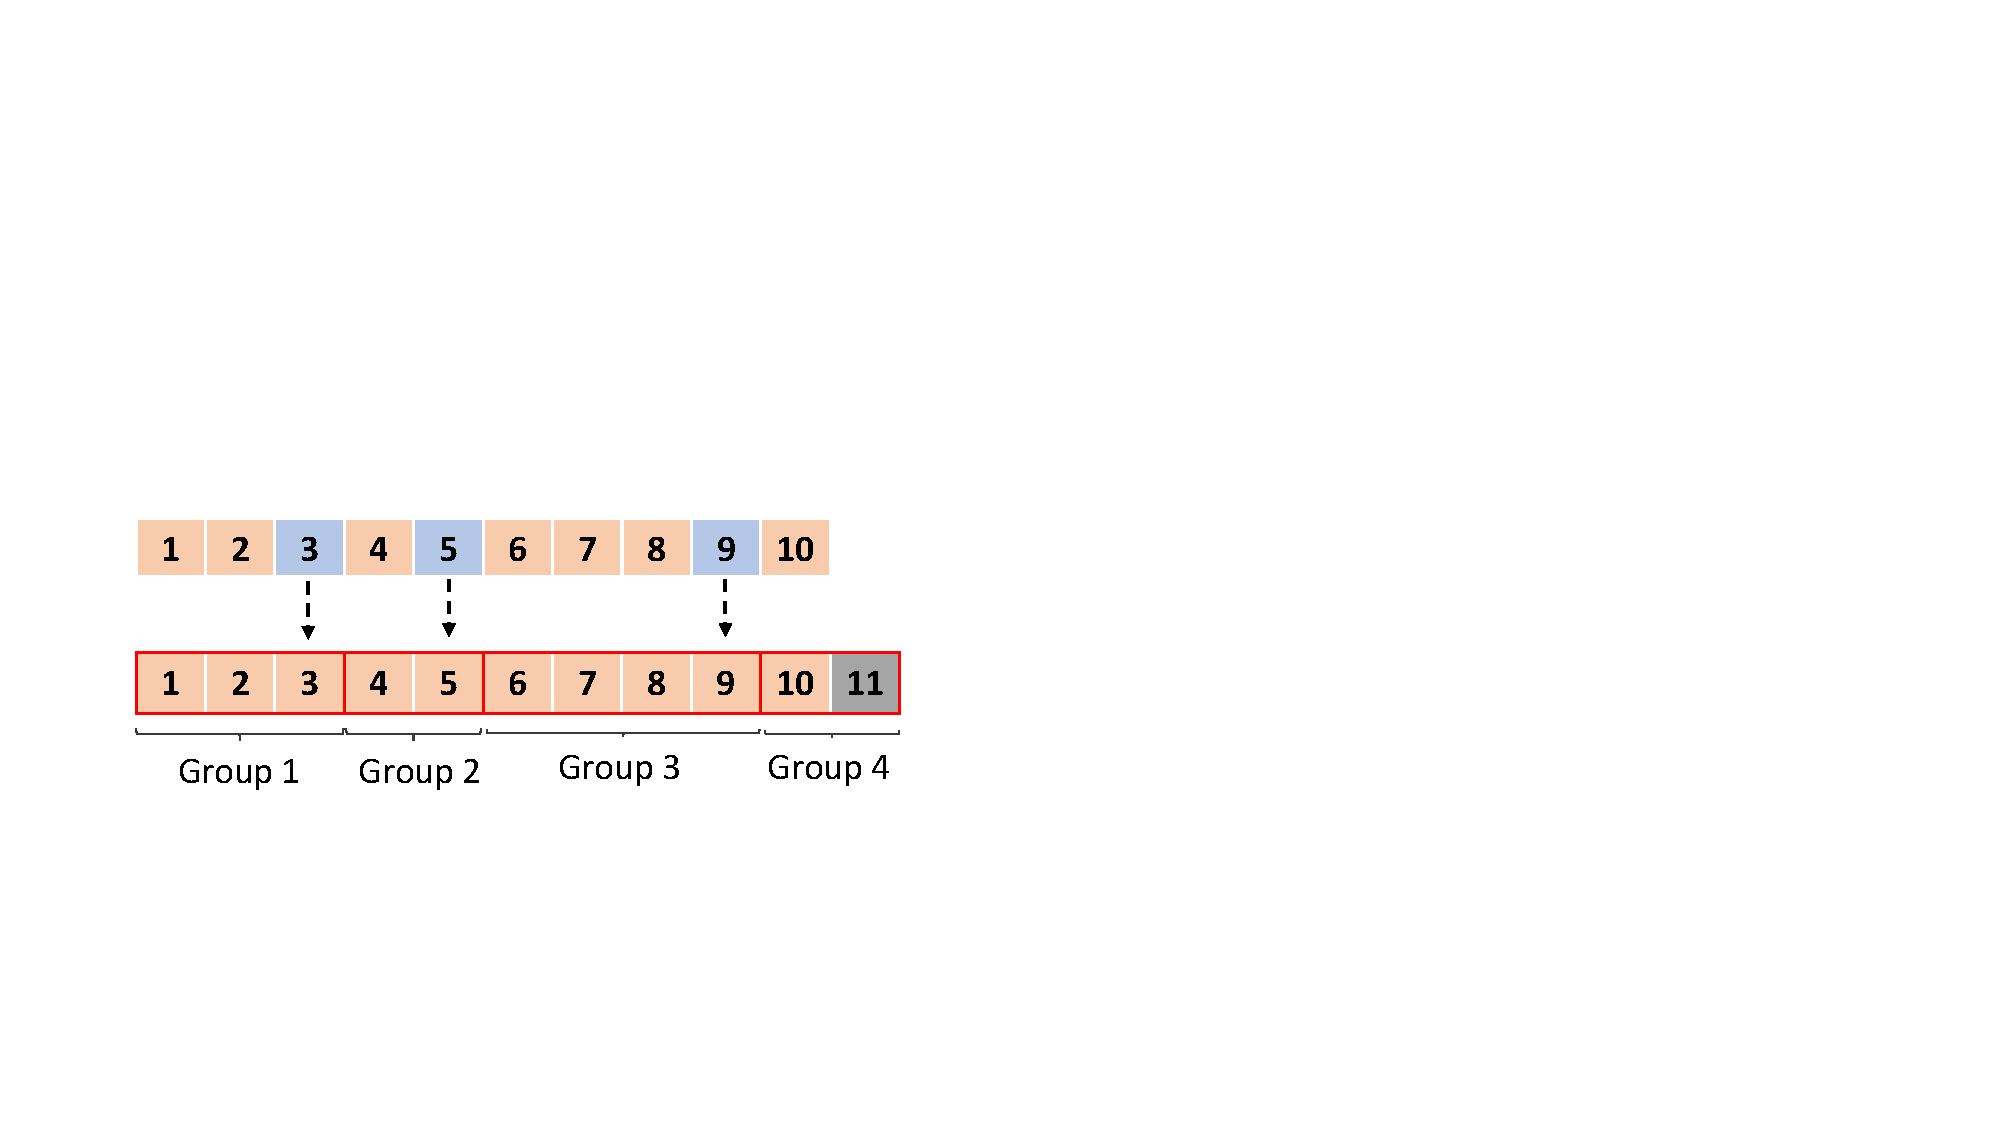
\includegraphics[width=0.55\textwidth]{./Figures/illustration.pdf}
    \caption{Illustration of Groups with Social Distancing}\label{fex1}
\end{figure}

In the model, the size of the row is $L = L^{0} + \delta =11$. The seat plan for the row can be represented by $\bm{h} = (2,1,1,0)$ with %. The maximum number of individuals that can be accommodated is 
$|\bm{h}| = 7$.
%\end{example}

The seat planning with deterministic requests problem (SPDRP) can be formulated by an integer programming, where we define $x_{ij}$ to be the number of type $i$ planned in row $j$. 

\begin{align}
(\textup{SPDRP}): \max \quad & \sum_{i=1}^{M}  \sum_{j= 1}^{N} (n_i- \delta) x_{ij} \notag \\
\text {s.t.} \quad & \sum_{j= 1}^{N} x_{ij} \leq d_{i}, \quad i \in \mathcal{M}, \label{deter_upper}\\ 
& \sum_{i=1}^{M} n_{i} x_{ij} \leq L_j, j \in \mathcal{N}, \label{capa_con} \\
& x_{ij} \in \mathbb{N}, \quad i \in \mathcal{M}, j \in \mathcal{N}. \notag 
\end{align}

The objective is to maximize the number of individuals accommodated. Constraint \eqref{deter_upper} ensures the number of accommodated groups does not exceed the number of requests. Constraint \eqref{capa_con} stipulates that the number of seats allocated in each row does not exceed the size of the row.

By examining the monotonic ratio between the original group sizes and the adjusted group sizes, we can establish the upper bound of supply corresponding to the optimal solution of the LP relaxation of SPDRP. This is illustrated in Proposition \ref{sol_relax_deter} and will be utilized in the bid-price control discussed in Section \ref{policies}.

\begin{prop}\label{sol_relax_deter}
For the LP relaxation of \textup{SPDRP}, there exists an index $\tilde{i}$ such that the optimal solutions satisfy the following conditions: $x_{ij}^{*} = 0$ for all $j$, $i = 1,\ldots, \tilde{i}-1$; $\sum_{j} x_{ij}^{*} = d_{i}$ for $i = \tilde{i}+1,\ldots, M$; $\sum_{j} x_{ij}^{*} = \frac{L - \sum_{i = \tilde{i}+1}^{M} {d_i n_i}}{n_{\tilde{i}}}$ for $i = \tilde{i}$.
\end{prop}

In other words, the supply corresponding to the optimal solutions for group types $i$ (where $i > \tilde{i}$) exactly matches the demand of group type $i$. For group types $i$ (where $i < \tilde{i}$), the supply is zero. The supply for group type $\tilde{i}$ is determined by the remaining available seats.

\subsection{Seat Planning Composed of Full or Largest Patterns}\label{seat_planning_full_largest}
The seat plan obtained from \textup{SPDRP} may not utilize all available seats, as it depends on the given requests. To improve a given seat plan and utilize all seats, we aim to generate a new seat plan composed of full or largest patterns while ensuring that the original group type requirements are met.

\begin{definition}
Consider a pattern $\bm{h} = (h_1, \ldots, h_M)$ for a row of size $L$. We define $\bm{h}$ as a full pattern if $\sum_{i=1}^{M} n_i h_i = L$. Addtionally, we refer to $\bm{h}$ as a largest pattern if its size $|\bm{h}| \geq |\bm{h}^{\prime}|$, for any other feasible pattern $\bm{h}^{\prime}$.
\end{definition}

In other words, a full pattern is one in which the sum of the product of the number of occurrences $h_i$ and the size $n_i$ of each group in the pattern is equal to the size of the row $L$. This ensures that the pattern fully occupies the available row seats. A largest pattern is one that either has the maximum size or is equal in size to other patterns, ensuring that it can accommodate the maximum number of individuals within the given row size.

\begin{prop}\label{lem_pattern}
If the size of a feasible pattern $\bm{h}$ is $|\bm{h}| = qM + \max\{r-\delta, 0\}$, where $q = \lfloor \frac{L}{M + \delta} \rfloor$, and $r = L - q (M + \delta)$, then this pattern is a largest pattern.
\end{prop}

The size, $qM + \max\{r-\delta, 0\}$, corresponds directly to a largest pattern that includes $q$ group type $M$ and $r$ seats for one group type $(r-\delta)$ when $r>\delta$. However, the form of the largest pattern is not unique; there are other largest patterns that share the same size.

% According to the definition of the largest pattern, the size of any largest pattern is given by $qM + \max\{r-\delta, 0\}$.

When $r = 0$, the largest pattern $\bm{h}$ is unique and full, indicating that only one pattern can accommodate the maximum number of individuals. On the other hand, when $r > \delta$, the largest pattern $\bm{h}$ is full, as it utilizes the available space up to the social distancing requirement.

A concept closely related to the largest pattern is the maximum achievable occupancy rate, which will be discussed in Section \ref{impact_sd} regarding the impact of social distancing. When all rows of a given layout consist of the largest pattern, the layout achieves its maximum achievable occupancy rate. This rate is defined as:

$$\frac{\sum_{j}\phi(M, L_{j}; \delta)}{\sum_{j} L_{j}- N \delta},$$

where $\phi(M, L; \delta)$ represents the size of the largest pattern under $M$ and $L$. According to Proposition \ref{lem_pattern}, $\phi(M, L; \delta)$ is non-decreasing in $M$. This is because any largest pattern $\bm{h}$ under $M$ remains a feasible pattern under $(M+1)$, implying that $\phi(M, L;\delta) \leq \phi(M+1, L; \delta)$. Consequently, when $M$ increases while $L$ remains constant, the maximum achievable occupancy rate also increases.

\begin{example}
Consider the given values: $\delta = 1$, $L = 21$, and $M = 4$. The size of the largest pattern can be calculated as $qM + \max\{r-\delta, 0\} = 4 \times 4 + 0 = 16$. The largest patterns are as follows: $(1, 0, 1, 3)$, $(0, 1, 2, 2)$, $(0, 0, 0, 4)$, $(0, 0, 4, 1)$, and $(0, 2, 0, 3)$. Among these, $(0, 0, 0, 4)$ is the form referenced in Proposition \ref{lem_pattern}.

The following figure shows that the largest pattern may not be full and the full pattern may not be largest.
\begin{figure}[ht]
    \centering
        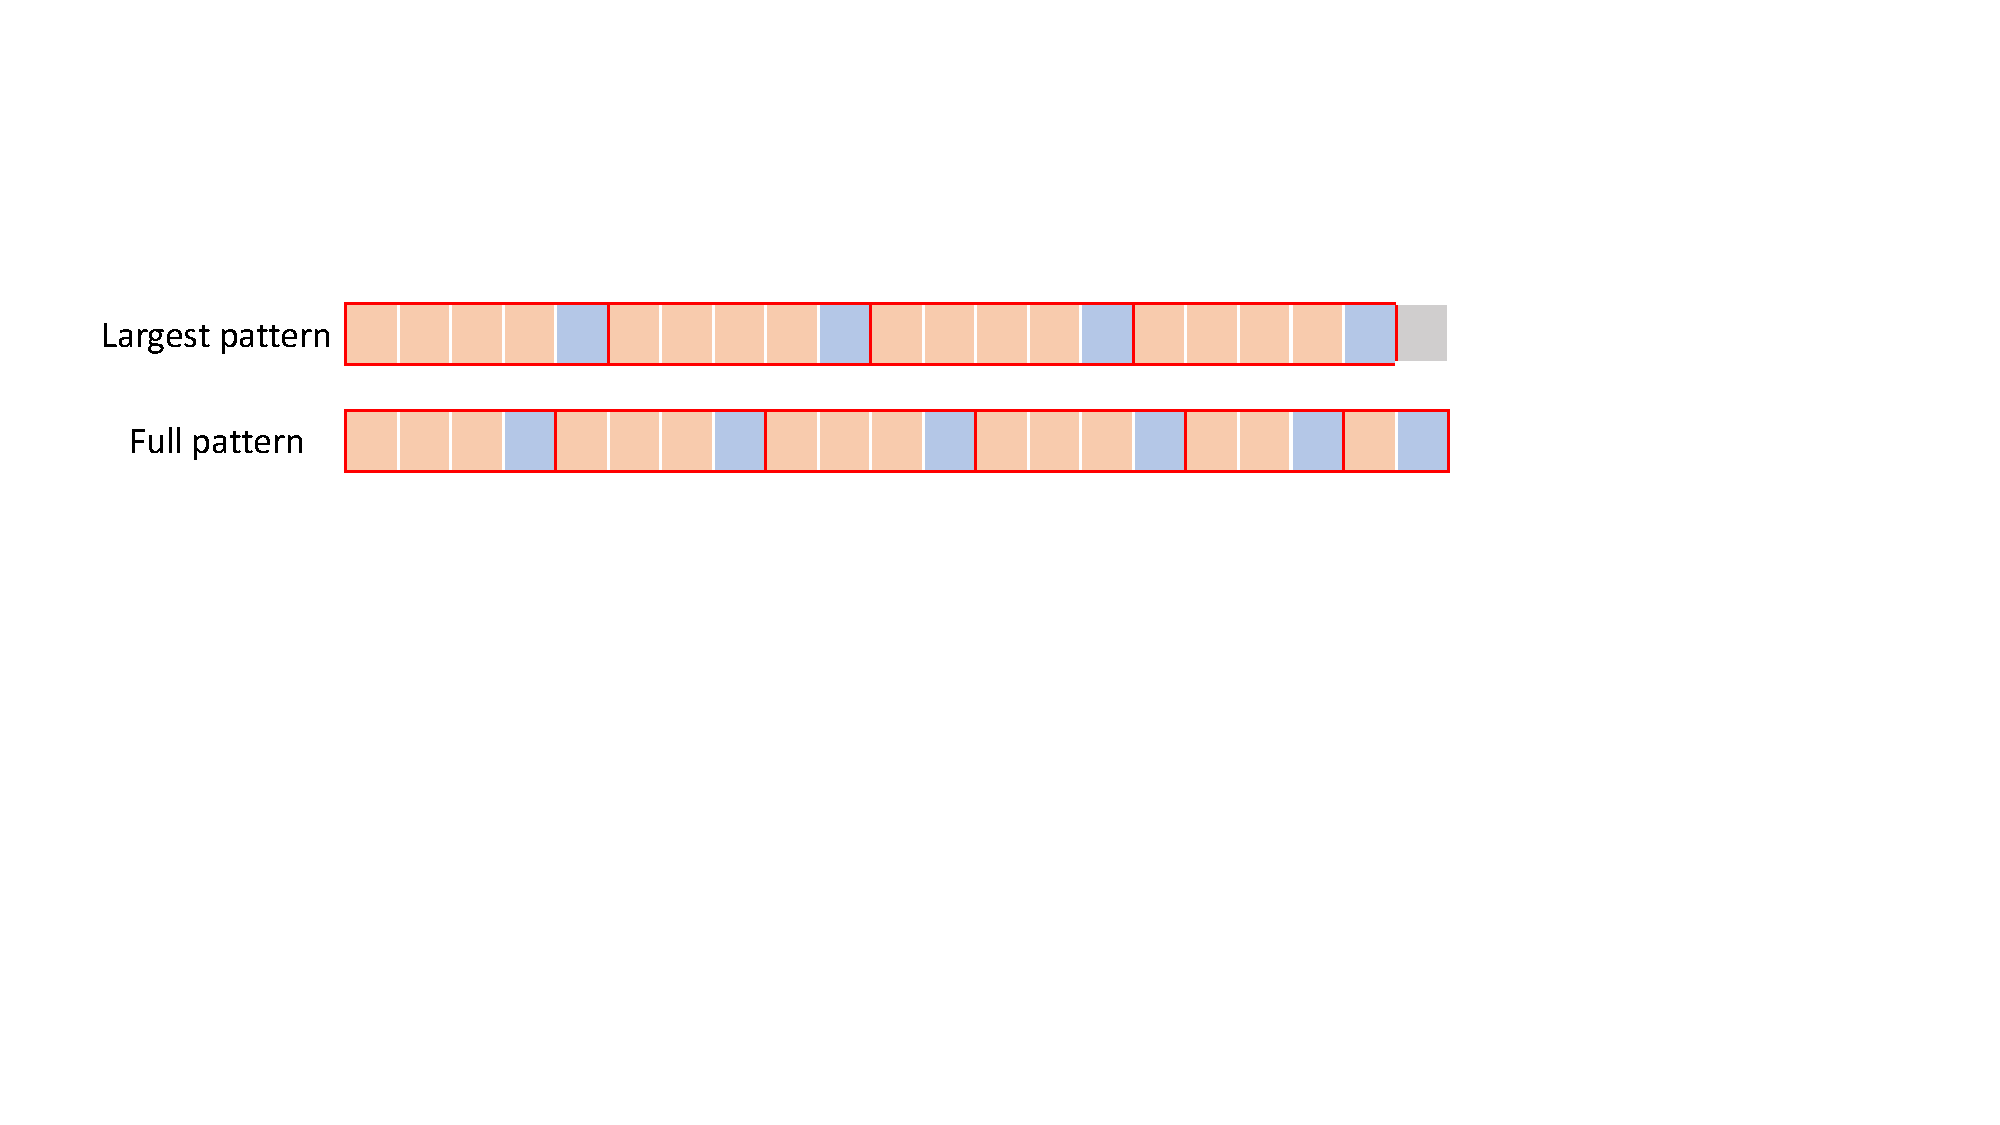
\includegraphics[width=0.8\textwidth]{./Figures/full.pdf}
    \caption{Largest and Full Patterns}
\end{figure}

The first row can be represented by $(0, 0, 0, 4)$. It is a largest pattern as its size is 16. However, it does not satisfy the requirement of fully utilizing all available seats since $4 \times 5 \neq 21$.
The second row can be represented by $(1, 1, 4, 0)$, which is a full pattern as it utilizes all available seats. However, its size is 15, indicating that it is not a largest pattern.
\end{example}

To obtain a seat plan composed of the full or largest patterns, we make the following statements.
Let the original seat plan be $\bm{H}$ and the desired seat plan be $\bm{H}^{\prime}$. To satisfy requirements for the original group types, the total quantity of groups from type $i$ to type $M$ in $\bm{H}^{\prime}$ must be at least equal to the total quantity from group type $i$ to group type $M$ in $\bm{H}$. Mathematically, we aim to find a feasible seat plan $\bm{H}^{\prime}$ such that $\sum_{k=i}^{M} \sum_{j=1}^{N} H_{jk} \leq \sum_{k=i}^{M} \sum_{j=1}^{N} H^{'}_{jk}, \forall i \in \mathcal{M}$. We say $\bm{H} \subseteq \bm{H}^{'}$ if this condition is satisfied.

To utilize all seats in the seat plan, the objective is to maximize the number of individuals that can be accommodated. Thus, we have the following formulation:

\begin{equation}\label{improve_seat}
  \begin{aligned}
  \max \quad & \sum_{i=1}^{M} \sum_{j=1}^{N} (n_i-\delta)  x_{ij} \\
  s.t. \quad & \sum_{j=1}^{N} \sum_{k=i}^{M} x_{kj} \geq  \sum_{k=i}^{M} \sum_{j=1}^{N} H_{jk}, i \in \mathcal{M} \\
  & \sum_{i=1}^{M} n_{i} x_{ij} \leq L_{j}, j \in \mathcal{N} \\
  & x_{ij} \in \mathbb{N}, i \in \mathcal{M}, j \in \mathcal{N}
  \end{aligned}
\end{equation}

\begin{prop}\label{prop_construction}
Given a feasible seat plan $\bm{H}$, the solution to problem \eqref{improve_seat} corresponds to a seat plan $\bm{H}^{\prime}$ such that $\bm{H} \subseteq \bm{H}^{\prime}$ and $\bm{H}^{'}$ is composed of full or largest patterns.
\end{prop}


This approach guarantees efficient seat allocation by constructing full or largest patterns while still accommodating the original groups' requirements. Furthermore, the improved seat plan can be used for the seat assignment when the group arrives sequentially.


